\documentclass[12pt, notitlepage]{article}
\usepackage[margin = 1in]{geometry}
\usepackage[english]{babel}
\usepackage[utf8]{inputenc}
\usepackage[table]{xcolor}
\usepackage{graphicx, booktabs, tikz, enumitem, dcolumn, pdfpages, csquotes}
\usepackage[font=normalsize]{caption}%,labelfont=bf
\usepackage{subcaption}

\usepackage{xr-hyper}
\usepackage[colorlinks = TRUE, allcolors = blue]{hyperref}
\externaldocument{appendix}

\renewcommand*\rmdefault{ppl}

\usepackage{setspace}
\setstretch{1.5}

\usepackage[]{titlesec}
    \titleformat*{\section}{\large\bf}
    \titleformat*{\subsection}{\normalsize\it}

% Bibliography
\usepackage[round]{natbib}
\setlength{\bibsep}{5pt}

\widowpenalty=10000
\clubpenalty=10000

\title{\Large Violence, co-optation, and postwar voting in Guatemala}
\author{}
\date{Word count: 10,860}

% \usepackage[none]{hyphenat}

\begin{document}

\maketitle
\thispagestyle{empty}

\vspace{30pt}

\begin{abstract}
\setstretch{1.1}

Wartime civilian victimization produces a counter-reaction against the perpetrator. However, this effect hinges on the creation of collective memories of wartime events. In many countries, former fighting actors and political elites try to redirect memories of wartime events through denial, propaganda, and co-optation. Previous works have ignored these aspects. I argue that the effect of violence is conditional on the capacity of local communities to build collective memories and bypass those efforts. I test this argument using local-level data from Guatemala. Results show that the effects of state violence on postwar voting depend on prewar exposure to political mobilization.

\end{abstract}
\setstretch{1.5}

\newpage
\setcounter{page}{1}

\section*{Introduction}

Conflicts leave deep scars in postwar societies, but they do not always do so the way it is usually implied.
We know that civilian victimization triggers a counter-mobilization against the perpetrator that lasts for a long time \citep{Balcells:2012aa, Lupu:2017aa, Fontana:2017aa, Rozenas:2017aa, Rozenas:2019aa}, but we are agnostic about the conditions that influence the way civilians remember violent events.
In many postwar contexts, fighting actors or political elites try to steer memories of wartime events to avoid a particular reaction by the population, particularly if wartime events could be harmful to them in terms of public support.
In Sri Lanka or Spain, for example, violence against civilians was denied, blamed on the opposite side, or interpreted as a necessary means to bring peace and national unity \citep{Seoighe:2017aa, Palomares:2004aa}.

The state is sometimes successful in covering up wartime events.
In Argentina, people only found out about the extent of the repression carried out by the dictatorship after its defeat in 1982 \citep{Robben:1995aa}.
Another related strategy to avoid counter-mobilization is the co-optation of local elites by state authorities or rebel groups.
In Mozambique, according to \citet{Finnegan:1992aa}, civilians who had been captives of Renamo did not show any grievances towards the \textit{majubas}, the local enforcers of Renamo, perhaps because of the personal and family links they shared.

Does wartime violence have different effects on political preferences depending on the exposure to propaganda or co-optation strategies?
The theoretical framework found in previous research is not able to answer this question, as past works do not usually account for any local factor that could mediate the long-term effect of civilian victimization.
Violence is assumed to have a homogenous effect across different communities.
This omission makes it difficult to evaluate how active efforts by the political actors involved define the actual consequences of violence.

This paper tries to address this limitation.
I argue that the effect of wartime violence is the product of the construction of collective memories, which is influenced both by the perpetrator's efforts to stave off blame on wartime atrocities and by the capacity of local communities to build the collective memories that lead to counter-mobilization.
In particular, the local ideological context enables local communities to form a political interpretation of violent events that determines the effect of victimization on political preferences.

I focus on the case of Guatemala, which is a good example of the use of denying and cooptation strategies.
In the aftermath of the victimization campaign that took place in the early 1980s, the state tried to deny war events, set up a discourse that justified military actions as a necessary step to bring peace to the country, and forcefully recruited civilians into paramilitary units of local defense.
In a country where many areas had been isolated from national politics and where political illiteracy was rampant, this strategy was to a large extent successful.
Some of the areas that were most brutally hit by state violence during the early 1980s became years later the electoral strongholds of the right-wing political party led by the same dictator who had ordered many of the killings \citep{Ball:1999ab}.

The same process was not present everywhere.
Some communities had been exposed to leftist political mobilization in the years before the most violent phase of the war.
I argue that this exposure made them more resilient to the co-optation efforts of state authorities and the discoursed imposed by the government.
Prewar political mobilization provided these communities with a better understanding of political divisions and shaped local reactions to violence, which translated into increased electoral support for the former rebels.

Using extensive local-level data, I show that state-led violence against civilians had different effect on postwar voting for the URNG and the FRG, the two parties linked to the former guerrilla and the military regime of the early 1980s, respectively.
In particular, proxying prewar mobilization with two measures of road accessibility, I show that in more accessible municipalities, and thus those that presumably were more exposed to political mobilization before the victimization campaign of the early 1980s, state violence is linked to an increase in electoral support for the URNG and a decrease in support for the FRG.
On the contrary, in isolated places with worse road infrastructures, state violence did not have any meaningful effect on postwar voting patterns.
Assuming that road accessibility determined how much exposure local communities had to external political actors, the results support my argument.
Complementing the empirical analyses, I show in a separate section qualitative evidence coherent with the accessibility assumption and each of the steps of the theoretical mechanism.

This paper contributes to the literature on the historical legacies of conflict \citep{Daly:2012aa, Weintraub:2015aa, Osorio:2018aa, Zhukov:2018aa, Osorio:2021aa} and the long-term effect of violence on preferences \citep{Balcells:2012aa, Lupu:2017aa, Fontana:2017aa, Rozenas:2017aa, Rozenas:2019aa} in three ways.
First, it highlights that the political reaction to wartime events is influenced by the efforts of political elites to steer memories of conflict and the capacity of individuals or communities to resist these efforts.
Second, I show that the effects of wartime violence on political preferences are not homogenous, but depend on the degree of political mobilization at the local level.
Finally, I offer new empirical evidence from a case that has received little attention in the literature, compared to other Latin American countries.

\section*{Long-term effects of civilian victimization}

An emerging research agenda explores the long-term effects of violence against civilians, finding evidence for the so-called backfiring effect: violence against civilians causes a rejection of the perpetrator's political identity in the long run.
Using data at the individual level, \citet{Balcells:2012aa} studies the long-term effect of violence in Spain.
\citet{Lupu:2017aa} do a similar study in Ukraine, tracking the inter-generational transmission of conflict-related preferences at the level of individuals.
Both these works find that violence produces a backfiring effect among those who suffered violence or their relatives.

Other works focus on local-level effects.
\citet{Balcells:2010ab} analyzes the effect of civilian victimization on local-level voting patterns in Catalonia, Spain, without finding conclusive results.
\citet{Fontana:2017aa} explore the effect of the Nazi occupation of Italy during World War II and find that Nazi violence increased local electoral support for communist parties many decades later.
\citet{Rozenas:2017aa} find that the forced deportations by Stalin that took place in Ukraine in the 1940s are linked to less support for pro-Russian political parties in the long run.

These works suffer from a few limitations.
Previous research has treated the process that leads from violent events to a change in political preferences in a too simplistic way, treating it as a black box.
A partial exception is \citet{Rozenas:2019aa}, who study the long-term effects of the Holomodor in Ukraine, and find that the effect of state repression is conditional on the structure of political opportunities.
In particular, opposition in communities exposed to repression was only visible during periods when the Soviet state could not credibly commit to repress contentious activities.

Focusing on Guatemala, the closest work to this paper is \citet{Vogt:2019aa}.
Using a similar research design, they show that state violence during the civil war in Guatemala led to higher electoral support for leftist parties in the postwar period.
They argue that the effect of violence should depend on the ``victims' embeddedness in their communities'' and show that the effect of state violence is more persistent in municipalities with a higher share of indigenous population.
However, linking the share of indigenous population to community cohesion is relatively problematic, particularly when some authors report fierce local conflicts and an increase of distrust in indigenous municipalities as a consequence of the counter-insurgency campaign \citep[e.g.][]{Burrell:2013aa}.
Moreover, both the concentration of state violence in indigenous areas and the coalition of the left-wing URNG with an explicitly indigenous party in 2011 and 2015 elections might explain part of this persistence in indigenous areas.
In any case, these findings are not at odds with the argument of this paper, and the role of social cohesion has more to do with the persistence of political identities than with their emergence as a result of violence.

All these works relatively ignore the local-level conditions of the effect of violence.
Individuals are assumed to objectively interpret violent events, and no attention is paid to those external factors that might influence this interpretation, such as propaganda or co-optation efforts by the perpetrator.
As \citet[1244]{Basta:2018aa} says, ``scholars usually take the meaning of events for granted, examining their causal efficacy without accounting for the processes of political contestation through which this meaning is created.''
Little theoretical attention has been paid to those local conditions that might explain the heterogeneous effects of violence.

This paper tries to overcome this limitation.
I assume that the process leading from violent events to a change in political preferences is not a direct, homogenous one.
The translation of wartime events into a change in preferences depends on the political interpretation of these events and the creation of collective memories of the conflict.
Efforts by the perpetrator in changing the interpretations and thus steering collective memory can effectively alter the response to wartime events.
Previous research has shown that different individuals can hold very different views of the same wartime events \citep{Driscoll:2016aa}, a variation that can follow political factors \citep{Silverman:2019aa}.

Moreover, the political response to events involves a social process of interpretation and remembering.
Individuals cope with trauma collectively \citep{Lyons:1998aa}, sharing their interpretations of wartime events and the political response to them.
The type of political interpretations an individual is faced with in face-to-face interactions is probably a more important determinant of her political response to these events than the events themselves \citep{Dyrstad:2012aa, Molina:2014aa, Glaurdic:2016aa}.
My theoretical argument thus hinges on the idea that the local ideological context will determine the local creation of collective memories.
This idea speaks to previous research on the role of social contexts in the persistence of political attitudes \citep{Wittenberg:2006aa, Tavits:2013aa}.

\section*{Historical context}

The Guatemalan civil war formally started in 1960 when a group of young officers led a revolt against the US-sponsored government.
The rebel officers approached the urban leftist movement and formed a guerrilla group based in the rural areas in eastern Guatemala \citep{Arias:1992aa}, ruling out the Maya population as a potential base of social support \citep{Smith:1990ab}.
The conflict remained at a low intensity for the next years, until a successful counterinsurgency campaign put down the insurrection in the late 1960s.
Many of the rebel leaders fled into exile.

Parallel to these events, the Guatemala countryside was rapidly changing.
The Catholic Action movement started to develop strongly during the 1960s.
The foreign Catholic clergy linked to the Liberation Theology expanded throughout the country, bringing new ideas and a new style of Pastoral work that criticized economic and political discrimination \citep{Arias:1992aa, Nelson:2009aa, Stoll:1999aa}.

The conflict entered a new phase in the 1970s.
Some of the defeated rebels joined forces with a younger generation and launched a new insurgency, this time with the idea of heading to the western highlands, the traditional homeland of the Maya.
The new guerrilla leaders identified the Indigenous population as a promising source of support, due to their age-old situation of political and economic discrimination \citep{Payeras:1981aa, Arias:1992aa}.
They tried to make contact with Catholic priests, although these contacts took place in an environment of mutual distrust \citep[e.g.][]{Manz:2004aa}.

The peasant movement was already fairly developed at this point.
It had emerged during the previous democratic period between 1944 and 1954 and, similar to Catholic Action, was fighting for land redistribution and the economic rights of the rural population \citep{Handy:1994aa, Forster:2001aa}.
It introduced new forms of economic organization and organized local political groups.
By the late 1970s, when the Committee for Peasant Unity (CUC) was formed, they were in contact with both the Catholic priests and the guerrilla.

With a guerrilla movement getting stronger and leftist mobilization expanding through the country, violence escalated quickly.
After 1980, all of the efforts concentrated on the armed struggle that was being waged by the four active guerrilla groups, which in 1982 merged into the URNG.
As the conflict entered a new phase, the Guatemalan government responded with a brutal counterinsurgency campaign.
The government focused on the civilian population that they thought constituted the base of support for the rebels, which for the most part were the rural Maya of the western highlands.
Violence intensified after 1978 and, by the early 1980s, reached genocidal levels.
More than 200,000 civilians were killed during the civil war, and over 90\% of the killings were committed by state forces \citep{Ball:1999aa, CEH:1999aa}.

Civilian victimization was first carried out in a relatively haphazard way under the regime of Lucas Garcia (1978--1982).
It later became more strategic under Ríos Montt (1982--1983), who engaged in a `scorched earth' campaign and sponsored a system to ensure compliance from the local population: the Civil Defense Patrols, or \textit{Patrullas de Autodefensa Civil} (PAC).
This system was ``established in virtually every municipio of the western highlands between 1982 and 1983'' \citep[272]{Smith:1990ab}.

The counterinsurgency campaign was successful.
Although it did not manage to end the conflict entirely, the strength of the rebel movement decreased significantly in the late 1980s and the war reached an impasse.
The peace talks finally culminated in a peace agreement signed in December 1996, and the guerrillas became a legal political party in 1998.
The war had ended, but its legacy endured in Guatemalan politics.\footnote{Among other things, the worsening situation in terms of violence that the country experienced after 1999 has been linked to the organizational legacies of the war combined with institutionalized state corruption, which also affects law-enforcement bodies such as the police \citep{Peacock:2003tt, Beltran:2016td, Booth:2010wd}. Some also link the presence of youth gangs to these dynamics \citep{Levenson:2013tm}.}

\section*{Violence, co-optation, and mobilization in Guatemala}

The victimization campaign of the early 1980s disrupted local communities. It pitted neighbors against neighbors and installed a climate of fear and distrust that would leave long-term consequences \citep{Burrell:2013aa}.
The government successfully destroyed Maya social organizations and gained forced cooperation from local people.
\citet[101]{Stoll:1999aa} tells how in ``Baja Verapaz, the army's reaction to CUC roadblocks was so savage that some of CUC's surviving members (...) changed sides and helped the army massacre one unarmed village after another.''

The PAC system was designed to ensure compliance within the countryside.
It forced local civilians to `defend' themselves from the guerrilla and, in many cases, successfully convinced them that they were on the good side and that violence and insecurity was the rebels' fault.
In more than a few instances, the PAC also assisted the army in massacring civilians.
The system aimed to destroy community networks and erode local interpersonal trust, which presumably had helped the guerrillas organize a local base of support \citep{SaenzdeTejada:2004aa}.
As \citet[641]{Bateson:2017aa} says, ``during the Guatemalan civil war, the military made a concerted effort to socialize and re-educate the civilians of the Western Highlands.''
The government explicitly recruited soldiers from the Maya communities into the army, including into the infamous Kaibil, the elite units that carried out many of the atrocities.
A woman described to \citet[112]{Green:1995aa} ``the particularly gruesome death of her husband at the hands of the army, while behind her on the wall prominently displayed was a photograph of her son in his Kaibil uniform.''

Beyond forced recruitment, the army also purposely establish a climate of fear, which ``made individuals more receptive to the military's propaganda, as they were desperate for some narrative to make sense of the chaotic, unpredictable violence surrounding them'' \citep[643]{Bateson:2017aa}.
The ideological warfare included rightist propaganda against communist ideas and any non-traditional form of social organization.
Ethnic identities were the target of the campaign as well.
Given that the Maya population eventually became the social base of support sought by the rebels, the ``program [was] based on eroding ethnic identity among Guatemala's Mayan Indian majority, and on brainwashing'' \citep[21]{Black:1985aa}.

This strategy had major consequences.
People from all across the political spectrum in Guatemala regarded the PAC system in particular as the most successful element of the army counterinsurgency campaign \citep{Garrard-Burnett:2010aa}.
The whole co-optation plan and the uncertainty that prevailed in the countryside during the 1980s helped convince the local population of the army's anti-rebel theses and left a long-term distrust for politics \citep{Green:1995aa}.

I argue that this strategy carried out by state authorities was key to understand the long-term consequences of victimization in Guatemala.
On the one hand, the strategy was in many cases successful in establishing a narrative favoring the state's discourse.
In these areas, the state managed to avoid being blamed for acts of wartime victimization.
On the other hand, the capacity of some communities to resist state propaganda and to build collective memories of the conflict explains why state-led victimization backfired in the long term.
My argument states that this resistance was possible in places that had been exposed to prewar leftist mobilization, as they had the ideological tools to interpret wartime events differently.

% A potential second mechanism explaining these heterogeneous effects discounts the importance of state propaganda.
% Instead of resisting propaganda and co-optation efforts, areas that had been exposed to prewar leftist mobilization could have judged state violence differently, precisely because of their leftist orientation.
% I develop this idea below.
% Both mechanisms are complementary and explain why state violence had diverging effects across different communities.

\subsection*{The role of prewar mobilization}

The propaganda and co-optation campaign of the government was successful in building an alternative discourse of the war and shaving off culpabilities in many areas.
But not in all of them.
Some communities were better prepared to confront it than others.
They had been more in contact with leftist ideas of political and economic discrimination, which equipped them to better understand the conflict and develop collective memories.
\citet[223]{Kobrak:2013aa} illustrates this argument, saying that ``living under army control, many guerrilla supporters learned to forget they had even been attracted to the struggle at all. But not in Colotenango.''
In that community, peasant organizations managed ``to challenge the mind-set of submission the army had tried to establish through the civil patrols'' \citep[226]{Kobrak:2013aa}.

Mainly two types of actors carried out these mobilization activities during the 1960s and 1970s.
On the one hand, Catholic Action priests inspired by Liberation Theology, which was already becoming a key political influence in Latin American \citep[e.g.][]{Wood:2003aa}.
In Guatemala, these religious activities took place throughout the countryside and had a clear political dimension \citep{Carmack:1988aa, Manz:1988aa, Manz:2004aa, LeBot:1992aa, Bateson:2013aa}.
On the other hand, a peasant movement developed parallel to the expansion of the Liberation Theology clergy, and both eventually intertwined.
Much of the work that Catholic priests carried out involved developing new forms of social and agricultural organization.
One of these was cooperativism, which had profound political consequences as it organized the local population and showed them alternative options to the existing economic and social regime \citep{Arias:1992aa, Nelson:2009aa, Bateson:2013aa}.

These activities were a key factor in developing ideological affinities in a country where many areas had not been exposed to political mobilization before.
As \citet[84]{Lofving:2005aa} affirms, ``in the population as a whole the absence of ideology and the presence of violence at the time loyalties were decided upon existed parallel to the presence of a defined cause in politically active circles.''
The consequences of the political mobilization carried out by these actors would not be limited to the conflict but also to the way people remembered it.

Communities with a previous history of political mobilization would have had interpreted information about the war and the reasons behind the violence differently.
Previous research points to how everyday social networks act as vectors of information during a conflict \citep{Shesterinina:2016aa} and influence the political reactions to past violence \citep{Rydgren:2007aa, Dorff:2017aa}.
I argue that communities that had been more exposed to this form of leftist mobilization before the war were more resilient to the co-optation strategies carried out by the government.
They were better equipped to understand what violence meant, to create collective memories of violent events, and to develop political identities as a response.

An alternative but complementary mechanism also explains the differences between communities without accounting for the role of state propaganda.
Previous research shows that the short-term effect of wartime violence on combatant support varies depending on whether the perpetrator is part of the in-group or not \citep{Lyall:2013aa}, as civilians evaluate wartime events according to their previous political orientation \citep{Silverman:2019aa, Pechenkina:2020ul}.
A left-leaning ideological context would determine the way local communities judge wartime events and assign blame.
Thus, even without taking into account propaganda and co-optation strategies by the state, areas that had been more exposed to prewar leftist mobilization should judge wartime state actions more negatively.
Although this mechanism mainly refers to short-term reactions during the conflict, it would not be daring to assume that these beliefs determined political preferences in the long run.

This mechanism hinges on an ideology-driven active judgment of state violence, but it is not at odds with the former discussion on the capacity of some communities to resist state propaganda, which is also driven by local ideology.
During the civil war, information about wartime events in Guatemala was likely very limited, so beliefs about wartime events were formed in a context of high uncertainty.
Along these lines, recent research suggests that rumor evaluation in wartime contexts is largely determined by surrounding social networks \citep{Schon:2021wf}.
Active judgment of wartime events is thus very much intertwined with the `narrative contests' that unfold in a situation where state actors are actively trying to spread misinformation about what happened during the war.

% In a study on postwar elections, \citet[749]{Daly:2019aa} says that ``the security gains attributed to the stronger belligerent offsets the belligerent's use of atrocities, allowing it largely to evade culpability for violence.''

\subsection*{Expectations on postwar voting}

% The empirical expectations rest on two ideas.
% First, the propaganda and cooptation campaign of the Guatemalan government successfully managed to steer collective memories and avoid a counter-mobilization to its use of violence.
% Second, the exception was those communities that had been exposed to leftist mobilization before the war and thus had the ideological tools needed to interpret the violence and create collective memories of it.

In the empirical analyses, I track the effects of wartime violence on postwar electoral support to two political parties: the URNG and the FRG.
While the URNG was the party that emerged out of the former guerrilla group, the FRG was the party founded by General Ríos-Montt in 1989 that represented the right-wing nationalism put forward by the army during the conflict.
Even though more parties might have a similar ideology to the URNG and FRG, these were the more representative of the wartime cleavage.

Following the argument, the expectation is that state violence during the conflict should have produced a counter-reaction in the form of increased support for the URNG and decreased support for the FRG, but only in those communities where they were able to interpret wartime events and form collective memories:

\begin{enumerate}[label={\bf H\arabic*:} , ref=H\arabic* , wide=0.5em, leftmargin=*]
  \item \label{h:URNG-mob} In municipalities exposed to prewar political mobilization, wartime violence against civilians increased long-term local support for the URNG.
  \item \label{h:FRG-mob} In municipalities exposed to prewar political mobilization, wartime violence against civilians decreased long-term local support for the FRG.
\end{enumerate}

On the contrary, in communities that had not been exposed to prewar leftist mobilization, the state should have been able to successfully co-opt the local population and avoid being blamed for the violence.
The implication is that violence did not have any effect or even that it had the opposite one: increased support for the FRG and a rejection of the URNG:

\begin{enumerate}[label={\bf H\arabic*:} , ref=H\arabic* , wide=0.5em, leftmargin=*]
  \setcounter{enumi}{2}
  \item \label{h:URNG-no-mob} In municipalities not exposed to prewar political mobilization, wartime violence against civilians decreased long-term local support for the URNG.
  \item \label{h:FRG-no-mob} In municipalities not exposed to prewar political mobilization, wartime violence against civilians increased long-term local support for the FRG.
\end{enumerate}

The quantitative analyses can only offer limited evidence on the mechanisms discussed above.
In a separate section below, I discuss qualitative evidence in support of the assumptions of the argument and the proxy variables used.

\section*{Empirical design}

I build a local-level dataset covering all 325 municipalities in Guatemala across the 22 departments.\footnote{Although Guatemala currently has 340 municipalities, the sample is reduced because of the territorial changes that municipalities have experienced since 1970. See Appendix~\ref{app:muni}.}
With this setup, I analyze the effect of wartime violence against civilians committed by state authorities on postwar electoral support for the URNG and FRG, adding an interaction term for the level of prewar exposure to leftist mobilization.

I run OLS models pooling observations from every municipality in all five general elections between 1999 and 2015, including election-year fixed effects.\footnote{I show results for separate cross-sectional models on each election in Appendix~\ref{app:results_year}.}
All models include department fixed effects to compare only municipalities within the same department.
Given that wartime violence was strongly concentrated in a few areas of the country, I also run the main models using a subset of the most affected departments.

\subsection*{Electoral results}

The main dependent variables are the share of votes to the URNG and the FRG in each election.
The URNG, which became a political party in 1998, was originally founded in 1982 as the umbrella group that included the four main rebel groups fighting against the government at the time.
The FRG was created in 1989 by General Efraín Ríos-Montt, the president of Guatemala between 1982 and 1983 who was behind much of the victimization campaign and designed the civil patrol system.
The FRG represented the anti-communist, right-wing nationalism that the army had sponsored during the war.
It still maintained the view that the conflict, and the violence it enfolded, had been the guerrillas' fault.\footnote{I also estimate models aggregating support for more political parties, both rightist and leftist, shown in Appendix~\ref{app:results_full}.}

Using data from the Supreme Electoral Tribunal \citep{TSE:2019aa}, I calculated the share of total valid votes received by each party in each municipality in every election between 1999 and 2015.\footnote{The FRG did not participate in 2011 elections. The URNG share includes its coalition partners: DIA in 1999; Winaq, ANN, and MNR in 2011; Winaq in 2015.}
Table \ref{tab:elec_results} shows the share of total votes received by both parties in each election.
Figure \ref{fig:map_elec1999} shows the geographical variation in support for each party in 1999 elections.

\begin{figure*}[!ht]
    \centering

    \begin{minipage}{1\textwidth}
      \centering
      \subfloat[URNG]
        {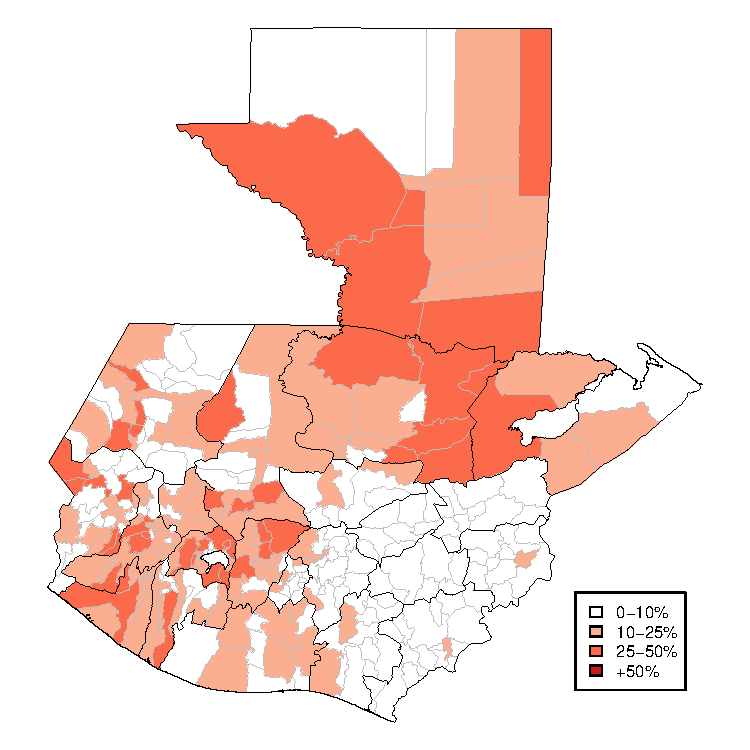
\includegraphics[width=0.4\textwidth]{img/map_URNG1999}}\hspace{25pt}
      \subfloat[FRG]
        {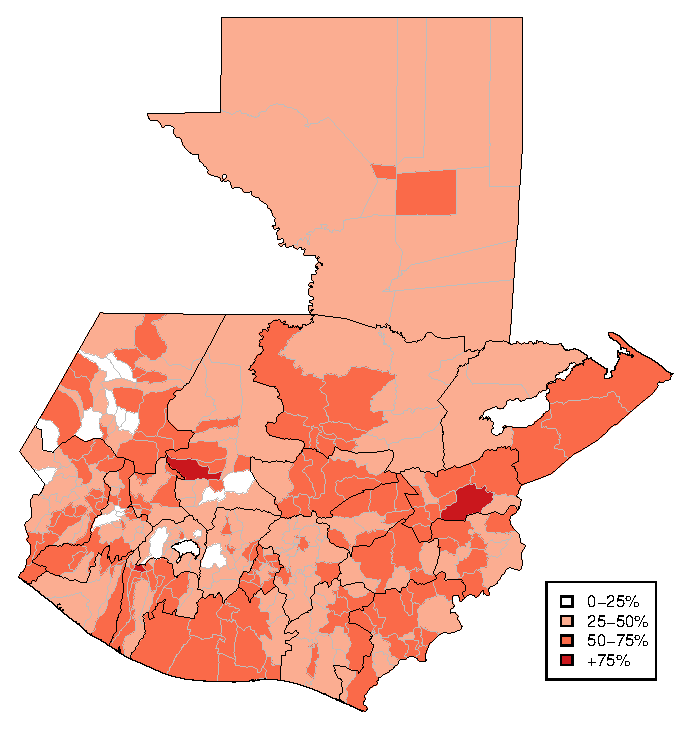
\includegraphics[width=0.4\textwidth]{img/map_FRG1999}}
    \end{minipage}

    \caption{Electoral results in 1999}\label{fig:map_elec1999}

\end{figure*}

\vspace{15pt}
\begin{table}[!htbp] \centering
  \caption{Electoral results of URNG and FRG}\label{tab:elec_results}
  \small

  \begin{tabular}{lccccc}
  \\[-1.8ex]\hline
  \hline \\[-1.8ex]
    & 1999 & 2003 & 2007 & 2011 & 2015 \\
  \hline \\[-1.8ex]
  URNG & 12.33\% & 2.58\% & 2.14\% & 3.26\% & 2.12\% \\
FRG & 47.75\% & 19.34\% & 7.3\% & -- & 0.87\% \\

  \hline
  \hline \\[-1.8ex]
  \end{tabular}

\end{table}

\subsection*{Civilian victimization}

To gather data on wartime violence against civilians I rely on and merge two different datasets, the records of the CEH and the \textit{Centro Internacional para Investigaciones en Derechos Humanos} (International Center for Human Rights Investigations, CIIDH), following previous research on political violence in Guatemala \citep{Chamarbagwala:2011aa, Sullivan:2012aa}.
Both CEH and CIIDH datasets are event databases built after extensive field research and together constitute a comprehensive picture of victimization events throughout the Guatemalan Civil War.

The CIIDH is a Guatemala-based NGO that carried out thousands of interviews and reviewed a variety of secondary sources to produce a list of more than 17,000 human rights violations by both sides, including more than 40,000 killings \citep{Ball:1999aa}.
The CEH was a UN-sponsored truth commission that focused on the massacres committed by the government against the civilian population and revealed that over 200,000 civilians were killed or disappeared during the conflict and that over 90\% of the killings had been committed by state authorities or related paramilitary groups \citep{CEH:1999aa}.
The CEH data was obtained from the replication data for \citet{Sullivan:2012aa}, who hand-coded massacres, defined as events of indiscriminate violence where at least 5 people were killed.
Combining both data sources offers a comprehensive picture of the conflict events in Guatemala.\footnote{I show in Appendix~\ref{app:results_ceh} that results do not change if only using data from the CEH.}

% Even though the CIIDH claims that its data are not a representative sample of wartime violent events, combining it with the CEH does offer a comprehensive picture of the conflict events in Guatemala.
% As \citet[382]{Sullivan:2012aa} explains, ``the three sources used to generate the CIIDH/CEH data (...) present a more accurate portrayal of the distribution of violence across Guatemala than any one source would have on its own.''\footnote{I show in Appendix~\ref{app:results_ceh} that results do not change if only using data from the CEH.}

Only events of fatal violence against civilians were selected and those whose location was unknown were removed (0.1\% of all events).
In the analyses, data on violence against civilians is limited to the period 1978--1985, which was by far the most violent period of the conflict.
I also include violence committed by the civil patrols, although the army participated in 98\% of the killings during this period.

For each municipality, I calculate the number of killings by state forces for every 1,000 inhabitants (using 1973 census data) and include it in the models in logarithmic form.
Figure \ref{fig:map_govt_vi} shows the geographical distribution of state violence.

\begin{figure*}[htb!]
  \centering
    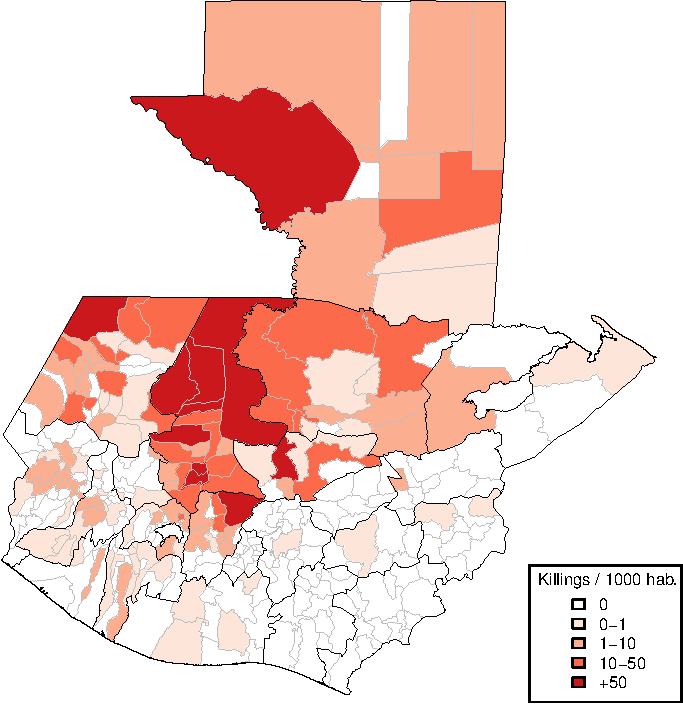
\includegraphics[width = .4\textwidth]{img/map_govt_vi}

  \caption{State violence against civilians in Guatemala, 1978--1985} \label{fig:map_govt_vi}

\end{figure*}

\subsection*{Proxying prewar mobilization}

Prewar exposure to political mobilization was a major factor determining the response of civilians to state violence in Guatemala.
Ideally, data on the presence and activities of leftist political actors before the most intense phase of the conflict would help to test this mechanism.
However, to my best knowledge, such data is not available.

Instead, I use two proxies for prewar exposure to political mobilization based on road infrastructure: distance to the Pan-American Highway, a major road-building project completed in the 1960s, and the share of non-paved roads in each municipality around 1970.
I assume that accessibility in terms of road infrastructure determined how much exposure local communities had to external political actors, who expanded throughout the country from the capital and main cities to bring new political ideas and organize the local population.
I provide further qualitative evidence supporting this claim in another section below.

The Pan-American Highway was a major US-sponsored development project completed in the 1960s.
The construction of the highway greatly improved communications.
This was particularly true in countries like Guatemala where former connections consisted of dirt roads or even mule trails, impassable during the rainy season.
The highway crosses Guatemala from West to East and extends through the heart of the western highlands.
The location of the route, originally planned to follow the Pacific coast, was chosen because of commercial reasons \citep{Rutkow:2019aa}.
The final construction of the highway brought about a great improvement in transportation in the early 1960s.
Precisely the moment in time when peasant associations and priests linked to the Liberation Theology began to expand throughout the country.

Municipalities closer to the Pan-American Highway should have had more exposure to prewar mobilization activities due to the easier logistics of arriving in these areas.
In other words, I assume that better transport infrastructure facilitated the continuous arrival of more political actors from Guatemala City and abroad.
I calculate how far away each municipality is from the road, and expect that municipalities closer to the Highway had a stronger exposure to leftist political mobilization during the 1960s and early 1970s.
Figure \ref{fig:map_panam} shows the distance between the boundary of each municipality and the Pan-American Highway (shown as a blue line), used in the analyses as $log(km + 1)$.

\begin{figure*}[htb!]
  \centering
    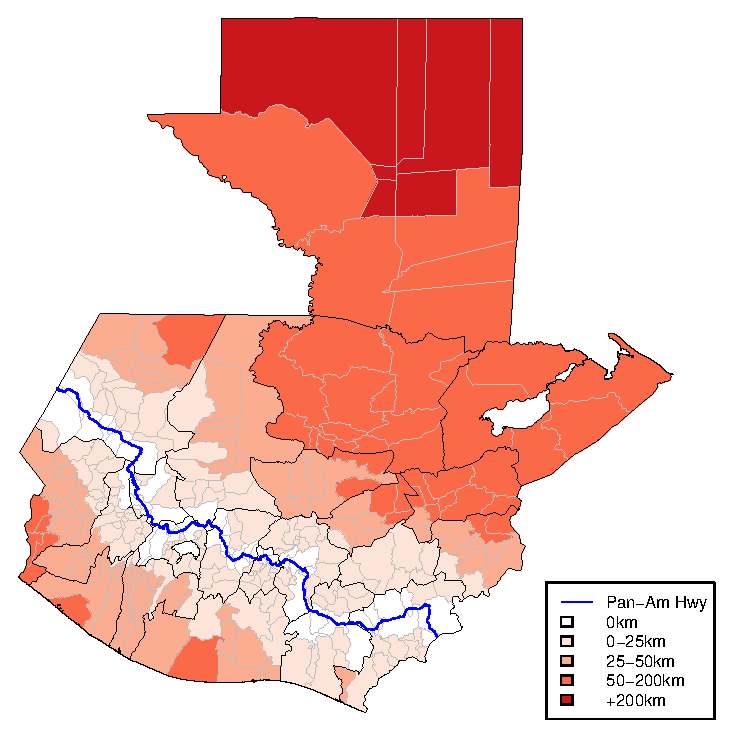
\includegraphics[width = .4\textwidth]{img/map_panam}

  \caption{Distance to Pan-American Highway} \label{fig:map_panam}

\end{figure*}

Distance to the Pan-American Highway provides more exogenous variation since the location of the highway did not respond to local political dynamics.
However, it might leave out some variation across municipalities further away from the highway.
Thus, I use a second proxy: the share of non-paved roads in each municipality.
Local road infrastructure would facilitate transportation within a community, thus leading to generally higher exposure to the activities of these actors.

Data comes from the National Geographic Institute of Guatemala \citep{Segeplan:2019aa} and corresponds to the road network based on raw information from the 1960s and 1970s.\footnote{Source: Email communication with the National Geographic Institute of Guatemala.}
It constitutes the best approximation for the period of interest, namely, road infrastructure right before the conflict escalated in the late 1970s.

The left panel (a) in figure \ref{fig:map_roads} shows the road network in Guatemala, with non-paved roads in grey and paved roads in black.
The right panel (b) shows the variable used in the analyses, the share of non-paved roads out of total road length.

\begin{figure*}[!ht]
    \centering

    \begin{minipage}{1\textwidth}
      \centering
      \subfloat[Road network ca. 1970]
        {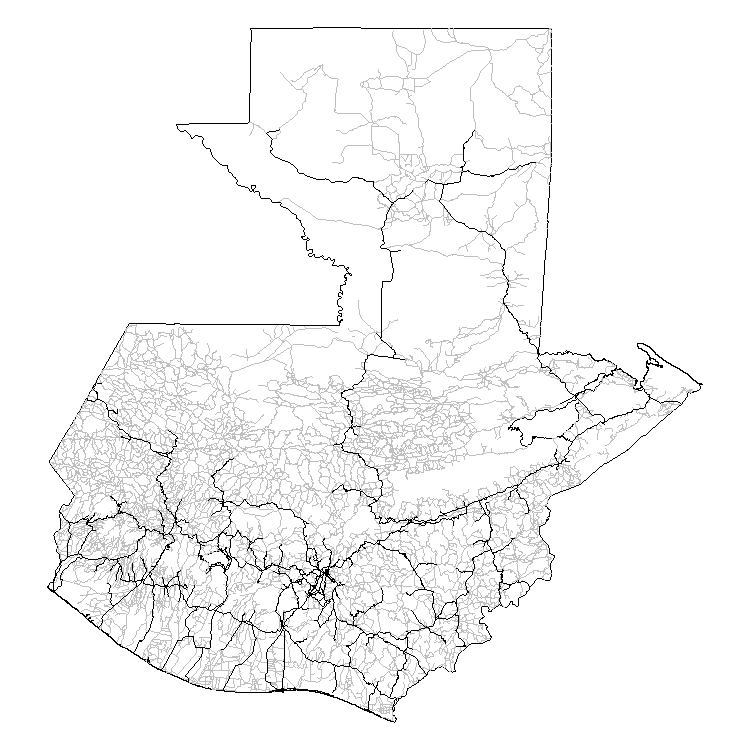
\includegraphics[width=0.4\textwidth]{img/map_roads}}\hspace{25pt}
      \subfloat[\% Non-paved by municipality]
        {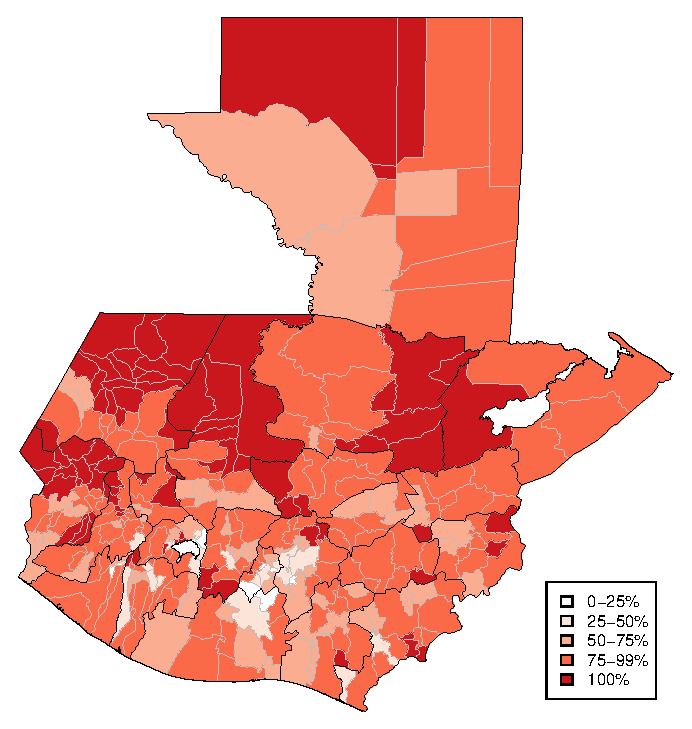
\includegraphics[width=0.4\textwidth]{img/map_roads_nonpaved_sh}}
    \end{minipage}

    \caption{Local road infrastructure} \label{fig:map_roads}

\end{figure*}


Neither of these two variables is correlated with patterns of state or rebel violence during the civil war, as I show in Appendix~\ref{app:lm_violence}.
The largest concern would be that accessibility drives rebel mobilization, which in turn would increase postwar electoral support for the rebels.
But the relationship between accessibility and rebel support through this mechanism would probably run the opposite way: state reach decreases in more isolated areas, facilitating rebel activity.
This bias would reduce the observed relationships.
Moreover, given that they are not highly correlated among them ($\rho = 0.23$), these two variables provide two different proxies for accessibility.

These variables introduce one potential alternative explanation related to state-building.
Namely, state violence did not have the same effect in isolated areas because of their lack of access to information and a general insularity from national politics.
Although I emphasize the importance of state propaganda and co-optation in driving political preferences in these areas, this explanation is not at odds with the theory.
My argument suggests that communities more accessible to the centers of power should be more familiar with political cleavages and thus have a higher `ideological capital.'
In other areas, lack of information and higher political illiteracy is probably part of the reason why the reaction to the violence was different, but at the same time, these factors also made it easier for the state to use propaganda and misinformation.

\subsection*{Controls}

Using data from the 1973 census, obtained from the replication data for \citet{Sullivan:2012aa}, I include the logged population of each municipality, the share of indigenous population, and the literacy rate.
I include two measures of terrain ruggedness: the standard deviation of elevation within each municipality, using data from the Digital Elevation Map of Guatemala \citep{Mapzen:2018aa}, and the share of forest cover from the GlobCover Land Cover Maps \citep{Arino:2012aa}.
I include a measure of rebel violence before 1978, the logged number of killings for every 1000 inhabitants following the CIIDH dataset \citep{Ball:1999aa}, to control for early rebel presence.
I also include the logged distance (km) from each municipality to Guatemala City and the logged area of each municipality (in $km^2$).
In Appendix~\ref{app:stats} I show that these variables are not strongly correlated among themselves, along with descriptive statistics.

\section*{Results}

Table \ref{tab:lm_base} shows the results of the base models, those that analyze the relationship between state violence and vote for the URNG and the FRG, in both the whole sample and only in the departments most affected by the violence.\footnote{Full tables in Appendix~\ref{app:results_tablong}.}
In every case the data pools together observations from all elections.
The first column (1) shows a positive relationship between state-led killings and URNG vote, but no relationship in the case of the FRG (2).


% Table created by stargazer v.5.2.2 by Marek Hlavac, Harvard University. E-mail: hlavac at fas.harvard.edu
% Date and time: Tue, Jul 27, 2021 - 13:56:47
% Requires LaTeX packages: dcolumn 
\begin{table}[!htbp] \centering 
  \caption{Base models on wartime violence and postwar voting} 
  \label{tab:lm_base} 
\small 
\begin{tabular}{@{\extracolsep{-20pt}}lD{.}{.}{-3} D{.}{.}{-3} D{.}{.}{-3} D{.}{.}{-3} } 
\\[-1.8ex]\hline 
\hline \\[-1.8ex] 
\\[-1.8ex] & \multicolumn{1}{c}{URNG} & \multicolumn{1}{c}{FRG} & \multicolumn{1}{c}{URNG} & \multicolumn{1}{c}{FRG} \\ 
 & \multicolumn{2}{c}{} & \multicolumn{2}{c}{\scriptsize Most affected departments} \\ 
\\[-1.8ex] & \multicolumn{1}{c}{(1)} & \multicolumn{1}{c}{(2)} & \multicolumn{1}{c}{(3)} & \multicolumn{1}{c}{(4)}\\ 
\hline \\[-1.8ex] 
 (Intercept) & 0.000 & 0.511^{***} & 0.021 & 0.448^{**} \\ 
  & (0.039) & (0.067) & (0.101) & (0.167) \\ 
  State-led killings & 0.007^{***} & -0.001 & 0.005^{+} & 0.001 \\ 
  & (0.002) & (0.003) & (0.003) & (0.004) \\ 
 \hline \\[-1.8ex] 
Controls & \multicolumn{1}{c}{Yes} & \multicolumn{1}{c}{Yes} & \multicolumn{1}{c}{Yes} & \multicolumn{1}{c}{Yes} \\ 
Department FE & \multicolumn{1}{c}{Yes} & \multicolumn{1}{c}{Yes} & \multicolumn{1}{c}{Yes} & \multicolumn{1}{c}{Yes} \\ 
Election FE & \multicolumn{1}{c}{Yes} & \multicolumn{1}{c}{Yes} & \multicolumn{1}{c}{Yes} & \multicolumn{1}{c}{Yes} \\ 
Observations & \multicolumn{1}{c}{1,601} & \multicolumn{1}{c}{1,281} & \multicolumn{1}{c}{491} & \multicolumn{1}{c}{394} \\ 
R$^{2}$ & \multicolumn{1}{c}{0.442} & \multicolumn{1}{c}{0.814} & \multicolumn{1}{c}{0.387} & \multicolumn{1}{c}{0.731} \\ 
Adjusted R$^{2}$ & \multicolumn{1}{c}{0.430} & \multicolumn{1}{c}{0.809} & \multicolumn{1}{c}{0.364} & \multicolumn{1}{c}{0.719} \\ 
\hline 
\hline \\[-1.8ex] 
\multicolumn{5}{c}{\parbox[t]{0.65\textwidth}{\textit{Note:} $+ p<0.1; * p<0.05; ** p<0.01; *** p<0.001$. All models pool all observations across all elections. Election and department FEs not shown. Most affected departments include Huehuetenango, Chimaltenango, Quiché, Alta Verapaz, Baja Verapaz, and Petén.}} \\ 
\end{tabular} 
\end{table} 


When looking at the most affected departments, the effect of state violence on leftist vote decreases, and it only stays significant at the 90\% level.
It suggests that the general trend found in the first model could indicate a concentration of both violence and leftist vote in the western highlands and Petén, rather than a robust relationship across the whole country.

Table \ref{tab:lm_panam} replicates the previous models but includes the interaction between state violence and distance to the Pan-American Highway.
In the case of URNG vote, the effect of state violence in municipalities contiguous to the highway is much stronger than in the base model.
The effect remains virtually the same in the sample limited to the most affected departments.
As the distance from the Pan-American Highway increases, the effect of state violence on leftist vote decreases.
Moreover, in the absence of violence, being closer to or further away from the highway does not have any effect on URNG vote.


% Table created by stargazer v.5.2.2 by Marek Hlavac, Harvard University. E-mail: hlavac at fas.harvard.edu
% Date and time: Thu, Jul 15, 2021 - 11:05:02
% Requires LaTeX packages: dcolumn 
\begin{table}[!htbp] \centering 
  \caption{Wartime violence, distance to PanAm Highway, and voting} 
  \label{tab:lm_panam} 
\small 
\begin{tabular}{@{\extracolsep{-20pt}}lD{.}{.}{-3} D{.}{.}{-3} D{.}{.}{-3} D{.}{.}{-3} } 
\\[-1.8ex]\hline 
\hline \\[-1.8ex] 
\\[-1.8ex] & \multicolumn{1}{c}{URNG} & \multicolumn{1}{c}{FRG} & \multicolumn{1}{c}{URNG} & \multicolumn{1}{c}{FRG} \\ 
 & \multicolumn{2}{c}{} & \multicolumn{2}{c}{\scriptsize Most affected departments} \\ 
\\[-1.8ex] & \multicolumn{1}{c}{(1)} & \multicolumn{1}{c}{(2)} & \multicolumn{1}{c}{(3)} & \multicolumn{1}{c}{(4)}\\ 
\hline \\[-1.8ex] 
 (Intercept) & 0.015 & 0.506^{***} & 0.052 & 0.433^{*} \\ 
  & (0.038) & (0.067) & (0.100) & (0.168) \\ 
  State-led killings & 0.024^{***} & -0.004 & 0.022^{***} & -0.003 \\ 
  & (0.004) & (0.006) & (0.005) & (0.009) \\ 
  Log. Dist to Pan-Am Hwy & 0.001 & 0.004 & 0.001 & 0.004 \\ 
  & (0.002) & (0.003) & (0.004) & (0.007) \\ 
  Violence $\times$ Dist to Pan-Am & -0.006^{***} & 0.001 & -0.006^{***} & 0.001 \\ 
  & (0.001) & (0.002) & (0.002) & (0.003) \\ 
 \hline \\[-1.8ex] 
Controls & \multicolumn{1}{c}{Yes} & \multicolumn{1}{c}{Yes} & \multicolumn{1}{c}{Yes} & \multicolumn{1}{c}{Yes} \\ 
Department FE & \multicolumn{1}{c}{Yes} & \multicolumn{1}{c}{Yes} & \multicolumn{1}{c}{Yes} & \multicolumn{1}{c}{Yes} \\ 
Election FE & \multicolumn{1}{c}{Yes} & \multicolumn{1}{c}{Yes} & \multicolumn{1}{c}{Yes} & \multicolumn{1}{c}{Yes} \\ 
Observations & \multicolumn{1}{c}{1,601} & \multicolumn{1}{c}{1,281} & \multicolumn{1}{c}{491} & \multicolumn{1}{c}{394} \\ 
R$^{2}$ & \multicolumn{1}{c}{0.453} & \multicolumn{1}{c}{0.814} & \multicolumn{1}{c}{0.407} & \multicolumn{1}{c}{0.732} \\ 
Adjusted R$^{2}$ & \multicolumn{1}{c}{0.441} & \multicolumn{1}{c}{0.809} & \multicolumn{1}{c}{0.382} & \multicolumn{1}{c}{0.718} \\ 
\hline 
\hline \\[-1.8ex] 
\multicolumn{5}{c}{\parbox[t]{0.65\textwidth}{\textit{Note:} $+ p<0.1; * p<0.05; ** p<0.01; *** p<0.001$. All models pool all observations across all elections. Election and department FEs not shown. Most affected departments include Huehuetenango, Chimaltenango, Quiché, Alta Verapaz, Baja Verapaz, and Petén.}} \\ 
\end{tabular} 
\end{table} 


These results can be more clearly seen in figure \ref{fig:pp_URNG_panam}, which shows the predicted effect of state violence on URNG vote in three municipalities located next to the highway, 20km away, and 400km away.
State violence has a positive impact on leftist vote in the first case, but it decreases and becomes negative as distance increases.
Assuming the variable is a good proxy for prewar mobilization, these results indicate that state violence only increased leftist vote in municipalities that had been exposed to political mobilization before the conflict intensified.

\begin{figure*}[htb!]
  \centering
    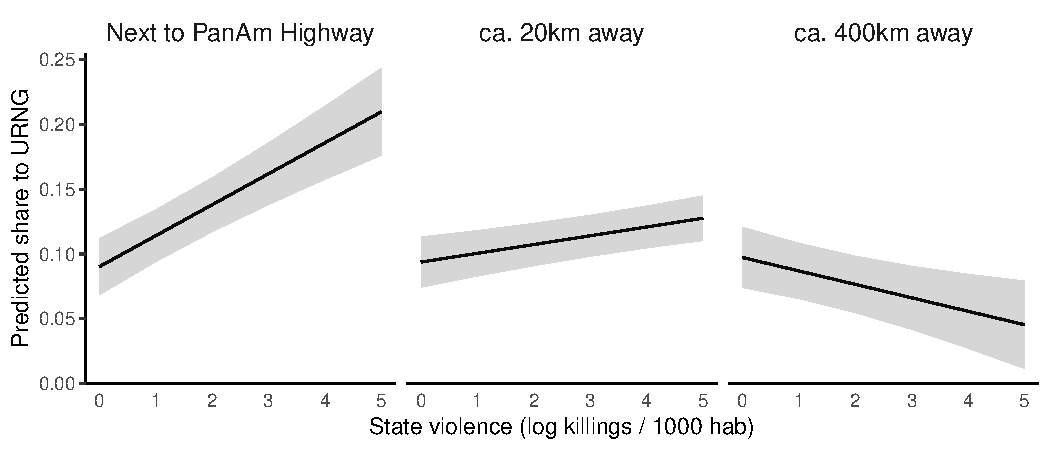
\includegraphics[width = .75\textwidth]{img/pp_URNG_panam}

  \caption{Wartime state violence and URNG share depending on prewar political mobilization (proxied by distance to Pan-American Highway), calculated for a municipality in Quiché, in 1999 elections, keeping all other variables at their mean, using Model 1 in Table~\ref{tab:lm_panam}.} \label{fig:pp_URNG_panam}

  % \vspace{5pt}
  % \raggedright
  % \scriptsize{Predicted share of URNG in the postwar period depending on wartime state violence and road infrastructure (distance to Pan-American Highway). Model includes department and election FEs. Predicted probabilities calculated for a municipality in Quiché, in 1999 elections, keeping all other variables at their mean.}

\end{figure*}

In the case of FRG vote, however, the results are not statistically significant.
State violence does not seem to have any meaningful effect, regardless of the value of the proxy for prewar mobilization.
Figure \ref{fig:pp_FRG_panam} illustrates this result, showing that, if anything, the results for the FRG go in the opposite direction than the models explaining URNG vote.

\begin{figure*}[htb!]
  \centering
    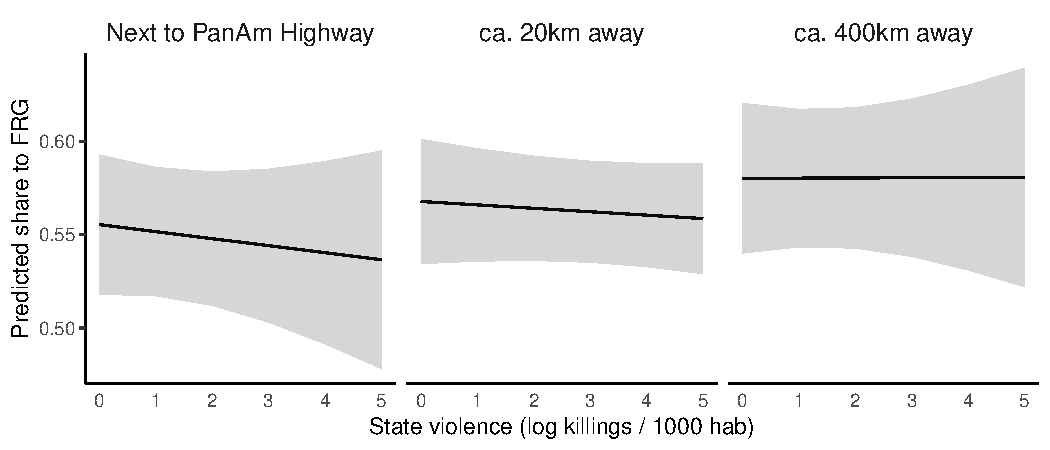
\includegraphics[width = .75\textwidth]{img/pp_FRG_panam}

  \caption{Wartime state violence and FRG share depending on prewar political mobilization (proxied by distance to Pan-American Highway), calculated for a municipality in Quiché, in 1999 elections, keeping all other variables at their mean, using Model 2 in Table~\ref{tab:lm_panam}.} \label{fig:pp_FRG_panam}

  % \vspace{5pt}
  % \raggedright
  % \scriptsize{Predicted share of FRG in the postwar period depending on wartime state violence and road infrastructure (distance to Pan-American Highway). Model includes department and election FEs. Predicted probabilities calculated for a municipality in Quiché, in 1999 elections, keeping all other variables at their mean.}

\end{figure*}

Table \ref{tab:lm_roads} shows the results for the same models but including the interaction with the local share of non-paved roads.
The results are stronger than those that use the first accessibility proxy.
State violence has a large positive effect on URNG vote in those municipalities which have all roads paved, and as the share of non-paved roads increases, the effect of state violence disappears.
In the most affected departments, the relationship is stronger and remains significant at the 99.9\% level.
The models on FRG vote share mirror these results but in the opposite direction, although the effect is only significant at the 95\% level.
State violence is linked to fewer votes for the FRG in municipalities where most roads are paved. As the share of non-paved roads increases, this effect disappears.


% Table created by stargazer v.5.2.2 by Marek Hlavac, Harvard University. E-mail: hlavac at fas.harvard.edu
% Date and time: Thu, Jul 15, 2021 - 11:05:02
% Requires LaTeX packages: dcolumn 
\begin{table}[!htbp] \centering 
  \caption{Wartime violence, local road network, and voting} 
  \label{tab:lm_roads} 
\small 
\begin{tabular}{@{\extracolsep{-20pt}}lD{.}{.}{-3} D{.}{.}{-3} D{.}{.}{-3} D{.}{.}{-3} } 
\\[-1.8ex]\hline 
\hline \\[-1.8ex] 
\\[-1.8ex] & \multicolumn{1}{c}{URNG} & \multicolumn{1}{c}{FRG} & \multicolumn{1}{c}{URNG} & \multicolumn{1}{c}{FRG} \\ 
 & \multicolumn{2}{c}{} & \multicolumn{2}{c}{\scriptsize Most affected departments} \\ 
\\[-1.8ex] & \multicolumn{1}{c}{(1)} & \multicolumn{1}{c}{(2)} & \multicolumn{1}{c}{(3)} & \multicolumn{1}{c}{(4)}\\ 
\hline \\[-1.8ex] 
 (Intercept) & -0.032 & 0.530^{***} & -0.158 & 0.602^{***} \\ 
  & (0.039) & (0.068) & (0.108) & (0.181) \\ 
  State-led killings & 0.044^{***} & -0.031^{*} & 0.081^{***} & -0.069^{*} \\ 
  & (0.007) & (0.013) & (0.017) & (0.028) \\ 
  \% Non-paved roads & 0.004 & 0.009 & 0.078^{*} & -0.042 \\ 
  & (0.009) & (0.016) & (0.038) & (0.064) \\ 
  Violence $\times$ Non-paved & -0.043^{***} & 0.034^{*} & -0.084^{***} & 0.077^{*} \\ 
  & (0.008) & (0.014) & (0.018) & (0.030) \\ 
 \hline \\[-1.8ex] 
Controls & \multicolumn{1}{c}{Yes} & \multicolumn{1}{c}{Yes} & \multicolumn{1}{c}{Yes} & \multicolumn{1}{c}{Yes} \\ 
Department FE & \multicolumn{1}{c}{Yes} & \multicolumn{1}{c}{Yes} & \multicolumn{1}{c}{Yes} & \multicolumn{1}{c}{Yes} \\ 
Election FE & \multicolumn{1}{c}{Yes} & \multicolumn{1}{c}{Yes} & \multicolumn{1}{c}{Yes} & \multicolumn{1}{c}{Yes} \\ 
Observations & \multicolumn{1}{c}{1,601} & \multicolumn{1}{c}{1,281} & \multicolumn{1}{c}{491} & \multicolumn{1}{c}{394} \\ 
R$^{2}$ & \multicolumn{1}{c}{0.453} & \multicolumn{1}{c}{0.815} & \multicolumn{1}{c}{0.415} & \multicolumn{1}{c}{0.737} \\ 
Adjusted R$^{2}$ & \multicolumn{1}{c}{0.440} & \multicolumn{1}{c}{0.810} & \multicolumn{1}{c}{0.390} & \multicolumn{1}{c}{0.723} \\ 
\hline 
\hline \\[-1.8ex] 
\multicolumn{5}{c}{\parbox[t]{0.65\textwidth}{\textit{Note:} $+ p<0.1; * p<0.05; ** p<0.01; *** p<0.001$. All models pool all observations across all elections. Election and department FEs not shown. Most affected departments include Huehuetenango, Chimaltenango, Quiché, Alta Verapaz, Baja Verapaz, and Petén.}} \\ 
\end{tabular} 
\end{table} 


These results are illustrated in figures \ref{fig:pp_URNG_roads} and \ref{fig:pp_FRG_roads}.
State violence has a large effect on leftist vote in more accessible municipalities.
When going from 0 killings to around 150 killings per 1000 inhabitants, the expected vote for URNG rises from 10\% to more than 30\%.
In the case of FRG vote, the effect goes in the opposite direction, less robust but still significant.
Violence decreases FRG vote in municipalities where most roads are paved, while it does not affect more isolated municipalities.

\begin{figure*}[htb!]
  \centering
    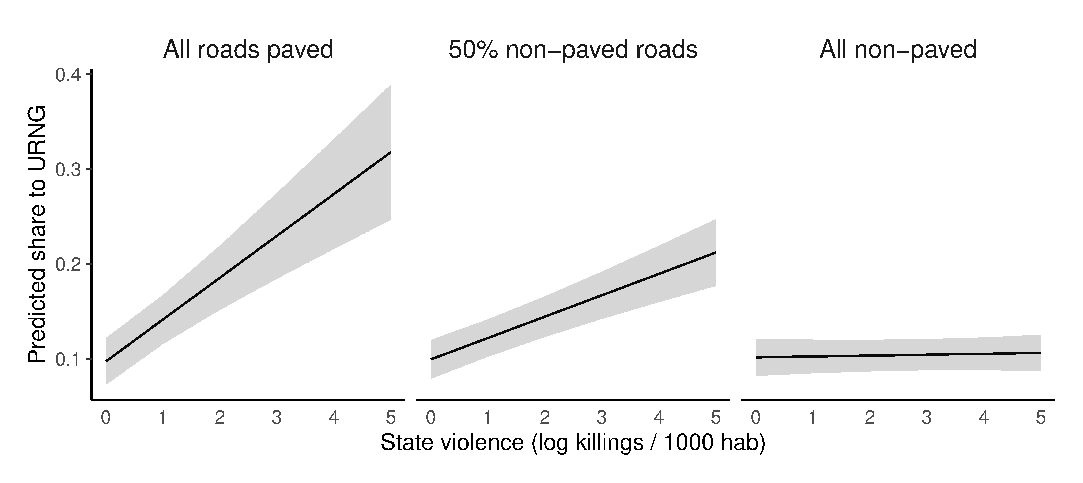
\includegraphics[width = .75\textwidth]{img/pp_URNG_roads}

  \caption{Wartime state violence and URNG share depending on prewar political mobilization (proxied by \% non-paved roads), calculated for a municipality in Quiché, in 1999 elections, keeping all other variables at their mean, using Model 1 in Table~\ref{tab:lm_roads}.} \label{fig:pp_URNG_roads}

  % \vspace{5pt}
  % \raggedright
  % \scriptsize{Predicted share of URNG in the postwar period depending on wartime state violence and road infrastructure (\% non-paved roads in a given municipality). Model includes department and election FEs. Predicted probabilities calculated for a municipality in Quiché, in 1999 elections, keeping all other variables at their mean.}

\end{figure*}

\begin{figure*}[htb!]
  \centering
    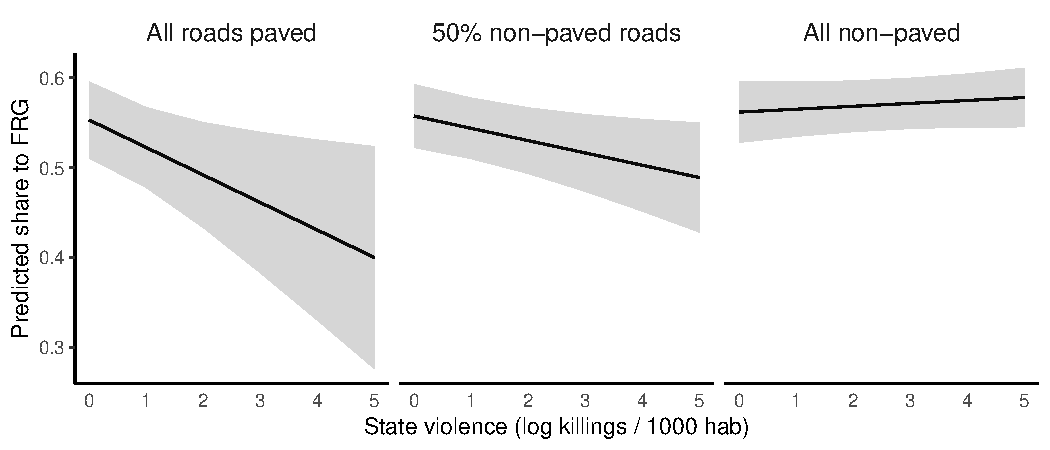
\includegraphics[width = .75\textwidth]{img/pp_FRG_roads}

  \caption{Wartime state violence and FRG share depending on prewar political mobilization (proxied by \% non-paved roads), calculated for a municipality in Quiché, in 1999 elections, keeping all other variables at their mean, using Model 2 in Table~\ref{tab:lm_roads}.} \label{fig:pp_FRG_roads}

  % \vspace{5pt}
  % \raggedright
  % \scriptsize{Predicted share of FRG in the postwar period depending on wartime state violence and road infrastructure (\% non-paved roads in a given municipality). Model includes department and election FEs. Predicted probabilities calculated for a municipality in Quiché, in 1999 elections, keeping all other variables at their mean.}

\end{figure*}

These findings are in line with the hypotheses outlined in the previous section, and particularly with those that refer to URNG vote (\ref{h:URNG-mob} and \ref{h:URNG-no-mob}).
In the case of the FRG hypotheses, the results are mixed.
The analyses provide empirical evidence for hypothesis \ref{h:FRG-mob}, which predicts a decreasing effect of violence on support for the FRG in municipalities more exposed to prewar mobilization.
However, hypothesis \ref{h:FRG-no-mob} is not directly supported by the data.

Results do not change if the independent variable measuring wartime violence only includes data from CEH (Appendix~\ref{app:results_ceh}) or when the dependent variable includes more parties (Appendix~\ref{app:results_full}).

In Appendix ~\ref{app:results_year} I also include results using a cross-section of the data for each election.
These results show that the effects of victimization was mainly present in the 1999 elections, and waned after that year.
In principle, this is coherent with the argument, since the difference between municipalities exposed to prewar mobilization and the rest should be, if anything, stronger right after the war and become less relevant after democracy was restored, for at least two reasons.
First, new issues different from wartime events emerged and increasingly defined voting patterns.
And second, new possibilities for political mobilization opened up, blurring the effect of the mechanisms discussed here.

Finally, an important source of concern in the use of the accessibility variables as proxies for the level of exposure to prewar mobilization is that these two proxies could be related to patterns of violence against civilians.
In Appendix~\ref{app:lm_violence}, I show that neither of these two variables is correlated with wartime violence by the state or the rebels.
If anything, the analyses show that wartime state violence was slightly more intense in municipalities further away from the Pan-American Highway.
Thus, none of the two proxies seems to be related to local conflict intensity.
I discuss this issue along with the details of the mechanism in the next section.

\section*{Identifying the mechanism}\label{sec:mechanism}

The empirical analyses do not test all the steps of the theoretical mechanism and hinger on the road accessibility assumption.
In response to these limitations, I provide in this section qualitative evidence identifying each step of the mechanism.
In particular, I discuss four main points: how the road infrastructure was a crucial factor explaining the diffusion of political mobilization in the years before the violence, the relationship between the presence of priests and activists and local mobilization activities, the role of state propaganda, and the existence of local commemoration activities in the postwar period.

% \subsection*{Road infrastructure and the diffusion of political activists}

First, there is qualitative evidence that road accessibility was related to political mobilization before the worst phases of the war.
In a study of Chupol, Chichicastenango, \citet{Esparza:2018uw} illustrates this point:

\begin{quote}
  for communities lying off the main road, facilitating the introduction of the new liberation theology gospel was the expansion of the Interamerican Highway in 1956. Chupolenses used the highway to increase their economic, social, and political networks throughout El Quiché. ... As their geographical isolation was now reduced by easier access to el pueblo and other adjacent townships, and particularly to Guatemala City, merchants both traveled to meet and were visited by outside institutions: rural Catholic Action catechists and Spanish and North American missionaries \citep[93--94]{Esparza:2018uw}.
\end{quote}

% Fn20, page 109: ``Later, on 16 August 1968, a second stage of the expansion of a new twenty kilometers of paved road from Los Encuestros to Chichi's town center introduced further social change for Chupolenses. CIRMA, El Imparcial, `Carretera: Encuestros Chichicastenango', 1, 4.''

Besides the role of these crucial actors and the importance of the Pan-American Highway, the argument states that accessible communities should have had more intense and continued contact with leftist activists.
Along these lines, \citet{Bran:1985tc}, writing in late 1980, explains that it was not only the main peasant or religious organizations that engaged in political mobilization, but also other types of local organizations that did not have explicit political goals but were also used as platforms for mobilization.
For example, he talks about a local soccer team where ``young revolutionaries make use of the weekly tours of regional championships to communicate with young peasants ... to exchange information, reading materials, ask for or offer help and other support activities for the organized popular movement'' \citep[15]{Bran:1985tc}.
It makes sense to expect that all these day-to-day activities would be more common in areas with better road connections.
Contrary to these areas, \citet{Esparza:2018uw} also discusses the so-called ``white communities'', those that were co-opted by the army and collaborated with the state.
``Among the poorest and those isolated from the Interamerican Highway, the army found a captive, obedient, and easily controlled support base to become complicit in the bloodshed'' \citet[138]{Esparza:2018uw}.

% \subsection*{Priests, activists and political mobilization}

Second, the role of priests and activists in leftist mobilization activities is also documented.
For instance, there are several reports of priests being expelled from the country because of political activities around the time of the 1974 elections \citep{Imparcial:1974ab, Imparcial:1974uz}.
One article published in late March 1974 affirms that these priests were expelled because of promoting local cooperatives in the department of Huehuetenango, and mentions six municipalities in particular where these activities took place: San Gaspar Ixchil, San Ildefonso Ixtahuacán, San Pedro Necta, San Rafael Petzal, Colotenango, and Santiago Chimaltenango \citep{Imparcial:1974aa}.

In table~\ref{tab:6muni}, I show these municipalities along with the number of victims that they later experienced in the early 1980s and the electoral share to the URNG in 1999.
Even though this is just anecdotal evidence, it is interesting to see that the two of them that experienced significant levels of victimization during the conflict (San Ildefonso and Colotenango) also reported high levels of support---above 40\%---for the former rebels in 1999, well above the nation-wide results (12.3\%).
Indeed, as mentioned above in the theoretical argument, \citet[223--226]{Kobrak:2013aa} explains that Colotenango was one of the municipalities that resisted the co-optation strategies carried out by the army precisely because of the strong presence of local peasant organizations.

\begin{table}[!htbp] \centering
  \caption{Huehuetenango municipalities mentioned in \citet{Imparcial:1974aa}}\label{tab:6muni}
  \small

  \begin{tabular}{lcc}
  \\[-1.8ex]\hline
  \hline \\[-1.8ex]
  Municipality & Victims in state violence & URNG share in 1999  \\
  \hline \\[-1.8ex]
  San Gaspar Ixchil & 0 & 13.4\% \\
  San Ildefonso Ixtahuacán & 228 & 42.3\% \\
  San Pedro Necta & 22 & 16.2\% \\
  San Rafael Petzal & 0 & 6.9\% \\
  Colotenango & 299 & 41.7\% \\
  Santiago Chimaltenango & 0 & 31.4\% \\
  \hline
  \hline \\[-1.8ex]
  \end{tabular}

\end{table}

% ``I define as `literate communities' those Chupol communities that were better prepared to consciously unmask the true goals of the army's civil action and psychological campaigns ... disseminating the internal enemy propaganda designed to compel peasants to join the patrol system'' \citep[92]{Esparza:2018uw}.
%
% Contrary to these areas, \citet[138]{Esparza:2018uw} highlights that
% Moreover, she also affirms that part of this cooperation was due to the lack of exposure to prewar mobilization activities, as ``poverty-ridden families from white communities refused to participate in the process of class and ethnic awakening led by Catholic Action, which encouraged participation in literacy projects and the use of new fertilizers and farming equipment'' \citet[139]{Esparza:2018uw}.

% \subsection*{The role of propaganda}

Third, both archival and qualitative evidence supports the idea that the state engaged in a strategy of propaganda that was in many cases successful.
For example, the army explicitly said in the \textit{Victoria 82} plan that one of their goals was ``to use the same procedures and techniques developed by the insurgency in the organization of the masses, since in this war the winner is the one who better organizes the people and has the greatest popular support.'' \citep[quoted in][II, 191]{CEH:1999aa}
By the late 1980s, when the war was waning and the first civilian president rose to power, the state was still involved in a full-fledged propaganda effort:

\begin{quote}
  Civil Affairs units continue to wage psychological propaganda operations of disinformation (OPSIC) by imputing blame on the guerrilla for the past destruction. Loudspeakers from helicopters and Civil Affairs patrols emphasize hardship for families, amnesty, and rewards for weapon turn-ins ... Leaflets dropped from airplanes and helicopters characterize the URNG as terrorists preying on peasants ... A radio OPSIC propaganda spot run every hour or so the week of President Cerezo's inauguration also fixed the blame for violence \citep[111]{Schirmer:1998wa}
\end{quote}

\citet[16]{Bran:1985tc} says that ``one of the most effective channels for the Guatemalan bourgeoisie to disseminate foreign and conservative ideologies among the people is the radio: falsified news, concealment of information, radio soap operas, official radio stations, ideologized messages, propaganda, etc.''
Contrary to the municipalities that had been exposed to leftist political mobilization, \citet{Esparza:2018uw} discusses how the army succeeded in co-opting local communities through a discourse based on demonizing the rebels and praising the army's development projects.

% \subsection*{Postwar commemoration activities}

Finally, one of the steps of the theoretical mechanism is that areas that had been exposed to prewar political mobilization were able to create their own collective memories of wartime events.
For this to happen, some form of commemoration activity is needed.
Qualitative sources also show evidence of these, even though a large part of the memory creation process probably took place in day-to-day interactions that were not recorded.
\citet{Falla:2006vu} describes how a Maya community in Ixcán, northern Quiché, could speak freely about past atrocities as they were free from military control.
Public discussion of wartime events allowed local people to challenge the army's misinformation campaign, particularly successful among younger people who had grown up away.

There are examples of more formal commemoration activities.
\citet{Arriaza:2008wf} talk about a few communities that established some form of local community museums to commemorate wartime massacres.
These local initiatives were of major importance to the creation of collective memories, particularly because ``in some communities, people have never spoken of what happened to them even within their own families'' \citep[161]{Arriaza:2008wf}.
Other accounts of local memorials also underscore the role they played in facilitating a collective discussion of wartime events.
For example, talking about a memorial cross built by a local community in Alta Verapaz, \citet[170--171]{Viaene:2011td} explains that the ``cross also created space for openly challenging and offering a counter-narrative against the army discourse that all the people who hid in the mountains were guerrilleros ... and therefore responsible for the atrocities.''

These activities, however, did not take place everywhere.
\citet{Viaene:2011td} talks about an isolated community in the same area that did not participate in the memorial construction, as both the army and the PAC enjoyed local control and had threatened local people.
\citet[178]{Esparza:2018uw} discusses the case of communities where militarization was intense and where ``collective fear of reprisals from former militia men continued to shape families' capacity to engage in grassroots action.'' In these communities, she affirms, ``the army replaced Indigenous peoples' shared memory with its own institutional memory'' (192).

% Moreover, the official commissions set up after the end of the war likely played a role in local contexts.
% Discussing the contribution of local activist groups to the truth commissions in the postwar period, \citet[123]{Esparza:2018uw} acknowledges that ``without these groups, the work of the commissions would not have successfully collected over 7,000 testimonies. ... Through locally based organizations, survivors with a past history with the politics of empowerment of the 1970s and 1980s were mobilized to provide information.''

\section*{Conclusion}

In many conflicts, political actors actively try to alter collective memories.
Propaganda, co-optation strategies, and local processes of mobilization define the political response to violence in each community.
In this paper, I point to the importance of these overlooked dynamics in understanding conflict legacies.

Using local-level data from Guatemala, I show that in many areas the government managed not to be blamed for the brutal campaign of victimization carried out during the civil war.
However, some communities had been exposed to leftist political mobilization right before the war.
They had acquired the ideological capital necessary to interpret violent events in political terms and were more resilient to state propaganda.
Contrary to other areas, in these communities state violence backfired in the form of long-term support for the rebels.

% This study offers novels insights that motivate future research and inform policy-making.
Even though this study focuses on Guatemala, the insights here motivate future research and inform policy-making.
The main takeaway is that we should take into account the social processes that determine the consequences of violence.
A better understanding of the social and political legacies of conflict is of major importance for postwar societies.
In these contexts, the main goal is to avoid a new outbreak.
Knowing how violence might have heterogeneous effects across different areas of the country can help to identify potential hot-spots of radicalization.
Moreover, the fact that memories of a conflict and the political responses to it are sensitive to the efforts of different political actors to change them can help to avoid such radicalization and to promote reconciliation.
A wrong reading of these findings would be that hiding facts could be a good strategy to avoid further violence.
But we do know little about how differential access to information about the conflict can bring about polarization, which constitutes a potential avenue for future research.
Instead, the discussion here suggests that peacebuilding programs should monitor the translation of collective memories into political responses and how these can lead to polarized identities.
In an unstable context, even a small fire can quickly grow in size and ignite another outbreak of violence.

\clearpage
\bibliographystyle{jpr}
\bibliography{REF}

% \newpage
% 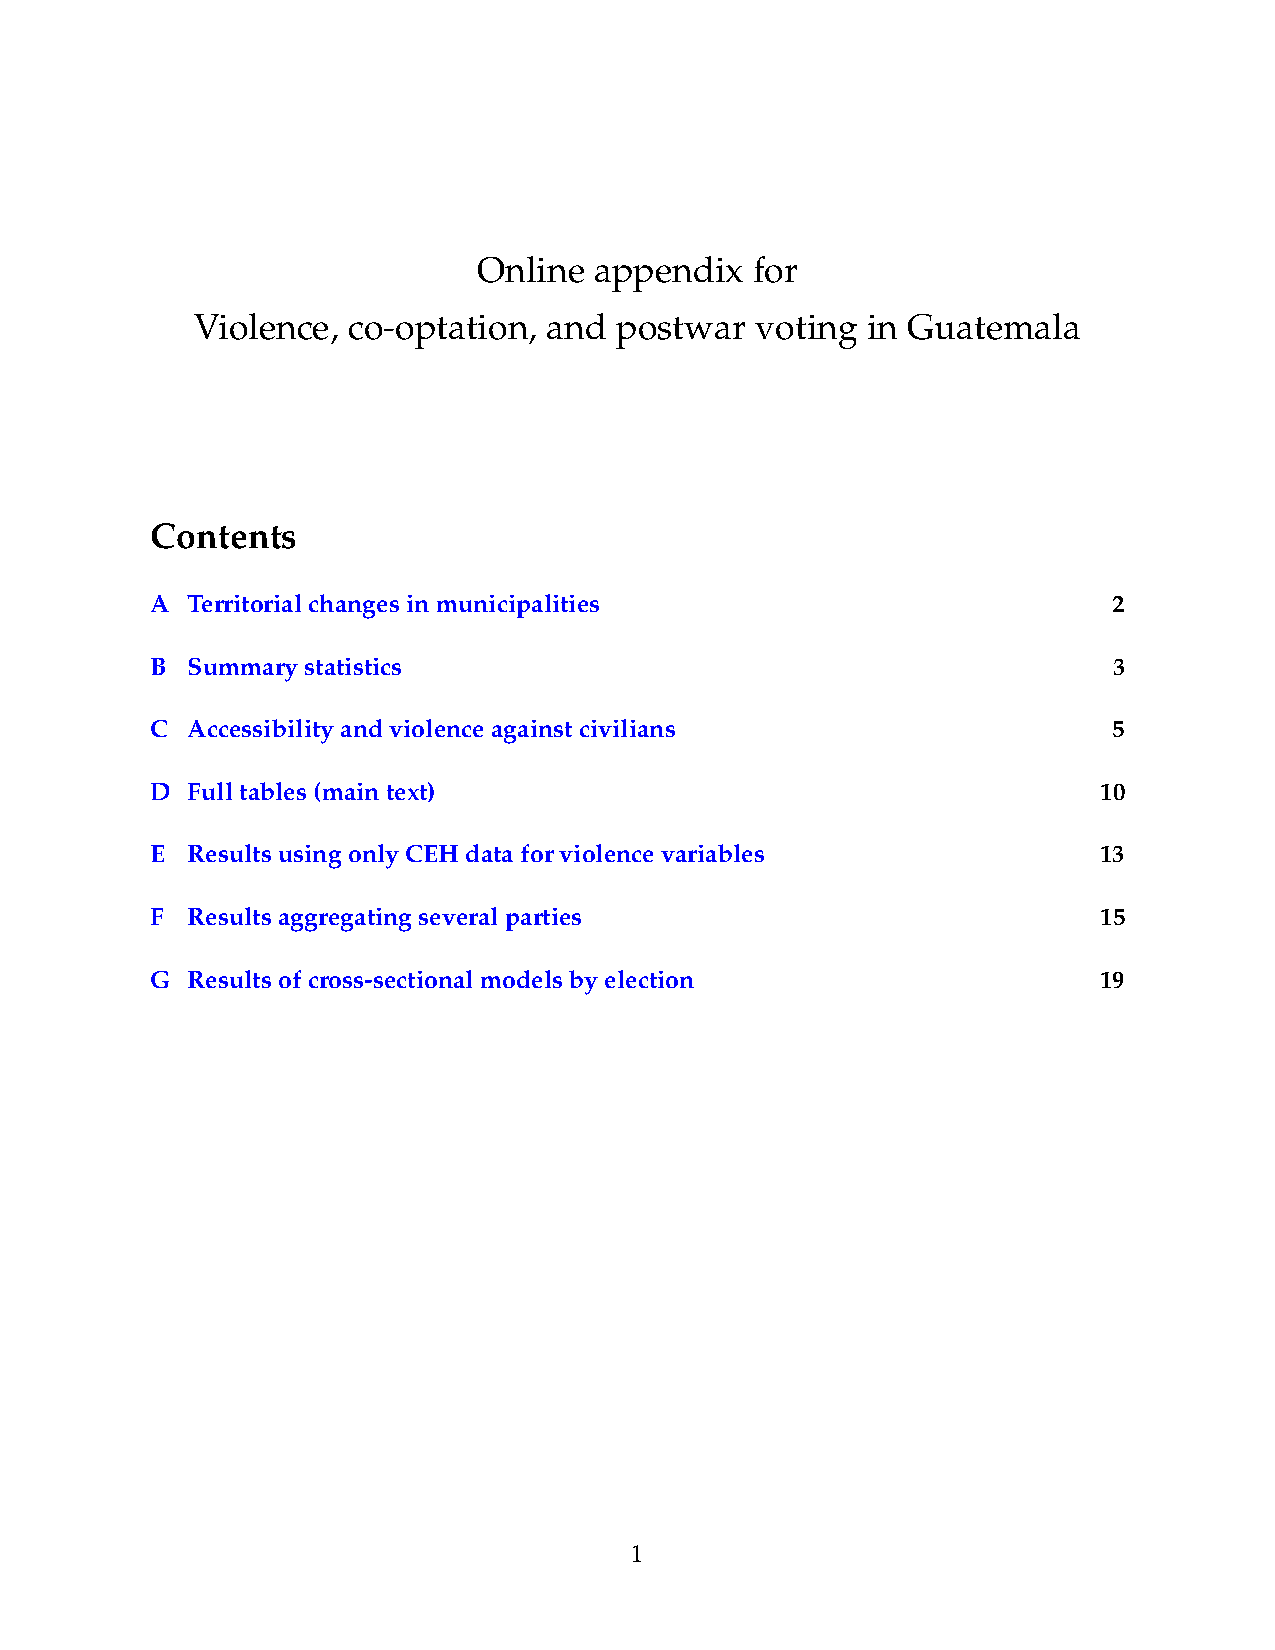
\includepdf[pages=-]{appendix.pdf}

\end{document}
